% !TEX encoding = UTF-8 Unicode
\documentclass[a4paper]{article}

\usepackage{color}
\usepackage{url}
\usepackage[T2A]{fontenc} % enable Cyrillic fonts
\usepackage[utf8]{inputenc} % make weird characters work
\usepackage{graphicx}

\usepackage[english,serbian]{babel}
%\usepackage[english,serbianc]{babel} %ukljuciti babel sa ovim opcijama, umesto gornjim, ukoliko se koristi cirilica

\usepackage[unicode]{hyperref}
\hypersetup{colorlinks,citecolor=green,filecolor=green,linkcolor=blue,urlcolor=blue}

\usepackage{listings}

%\newtheorem{primer}{Пример}[section] %ćirilični primer
\newtheorem{primer}{Primer}[section]

\definecolor{mygreen}{rgb}{0,0.6,0}
\definecolor{mygray}{rgb}{0.5,0.5,0.5}
\definecolor{mymauve}{rgb}{0.58,0,0.82}

\lstset{ 
  backgroundcolor=\color{white},   % choose the background color; you must add \usepackage{color} or \usepackage{xcolor}; should come as last argument
  basicstyle=\scriptsize\ttfamily,        % the size of the fonts that are used for the code
  breakatwhitespace=false,         % sets if automatic breaks should only happen at whitespace
  breaklines=true,                 % sets automatic line breaking
  captionpos=b,                    % sets the caption-position to bottom
  commentstyle=\color{mygreen},    % comment style
  deletekeywords={...},            % if you want to delete keywords from the given language
  escapeinside={\%*}{*)},          % if you want to add LaTeX within your code
  extendedchars=true,              % lets you use non-ASCII characters; for 8-bits encodings only, does not work with UTF-8
  firstnumber=1000,                % start line enumeration with line 1000
  frame=single,	                   % adds a frame around the code
  keepspaces=true,                 % keeps spaces in text, useful for keeping indentation of code (possibly needs columns=flexible)
  keywordstyle=\color{blue},       % keyword style
  language=Python,                 % the language of the code
  morekeywords={*,...},            % if you want to add more keywords to the set
  numbers=left,                    % where to put the line-numbers; possible values are (none, left, right)
  numbersep=5pt,                   % how far the line-numbers are from the code
  numberstyle=\tiny\color{mygray}, % the style that is used for the line-numbers
  rulecolor=\color{black},         % if not set, the frame-color may be changed on line-breaks within not-black text (e.g. comments (green here))
  showspaces=false,                % show spaces everywhere adding particular underscores; it overrides 'showstringspaces'
  showstringspaces=false,          % underline spaces within strings only
  showtabs=false,                  % show tabs within strings adding particular underscores
  stepnumber=2,                    % the step between two line-numbers. If it's 1, each line will be numbered
  stringstyle=\color{mymauve},     % string literal style
  tabsize=2,	                   % sets default tabsize to 2 spaces
  title=\lstname                   % show the filename of files included with \lstinputlisting; also try caption instead of title
}

\begin{document}

\title{Razvoj LSTM neuronske mreže i primena nad problemom sekvencijalnog učenja\\ \small{Seminarski rad u okviru kursa\\Računarska inteligencija\\ Matematički fakultet}}

\author{Nevena Soldat, Milena Kurtić\\ nevenasoldat@gmail.com, mimikurtic67@gmail.com}

%\date{9.~april 2015.}

\maketitle

\abstract{

}

\tableofcontents

\newpage

\section{Uvod}
\label{sec:uvod}
LSTM (eng. Long Short-Term Memory) je podvrsta rekurentne neuronske mreže. Rekurente neuronske mreže (eng. Recurrent Neural Networks - RNN) su specijalan tip neuronskih mreža koje se koriste za sekvencijalne probleme učenja. Eksperimenti su pokazali da je veoma teško trenirati rekurentne neuronske mreže efikasno. Naime, prilikom ažuriranja težina, može doći do toga da njihova promena bude toliko mala da nema efekta (vanishing gradient), odnosno toliko velika da su promene prevelike (exploding gradient). LSTM prevazilaze probleme klasičnih rekurentnih mreža. 

\subsection{Primena na vremenske serije}
Predviđanje vremenskih serija se može opisati kao proces koji izvlači korisne informacije iz vrednosti koje su se realizovale u nekom prethodnom trenutku, i na osnovu njih predviđa buduće vrednosti. Nailazimo na veliku primenu ove tehnike u oblastima poput vremenske prognoze, planiranja transporta, odnosno regulisanja saobraćaja. Metode predviđanja koje su bazirane na neuronskim mrežama stiču veliku popularnost jer je dokazano da mogu biti podjednako dobre kao klasične statističke metode. 

\section{Opis problema}
Cilj ovog rada je demonstriranje upotrebe LSTM neuronske mreže na problem predviđanja vremenskih serija. Kako je predviđanje toka pandemije virusa u trenutku pisanja ovog rada jedna od najektuelnijih tema, podaci koje koristimo predstavljaju broj obolelih, kao i broj žrtava zaraze ovim virusom.  
\subsection{Opis baze}
Za potrebe ovog projekta koršcena je baza podataka COVID19 Global Forecasting koja se u trenutku razvijanja ovog projekta svakodnevno ažurira. U njoj se nalaze podaci o broju osoba koje su potvrđeno zaražene virusom COVID-19, broju umrlih osoba koje su bile zaražene, datumi, pokrajne i države na koje se date brojke odnose. Podaci su smešteni u dva fajla test.csv i train.csv.   

\section{Rešenje problema}
Problem predviđanja toka pandemije virusa resavamo pomocu LSTM nerunske mreže. Program se sastoji iz sledecih delova:
\begin{itemize}
    \item \textbf{Pretprocesiranje}
    \item \textbf{Učenje modela nad trening podacima}
    \item \textbf{Testiranje modela}
\end{itemize}


\subsection{Pretprocesiranje}
Kako bismo primenili LSTM neuronske mreže moramo da sredimo podatke koje imamo. To, u ovom slučaju, podrazumeva popunjavanje nedostajućih vrednost kao i normalizaciju podataka.


Nedostajuće vrednosti imamo u koloni Province\_State. U svakom takvom slučaju u kom je vrednost iste kolone null, tu vrednost zamenjujemo sa vrednostima u koloni Country\_Region.  \ref{fig:Pretprocesiranje1}
\begin{figure}[htp]
    \centering
    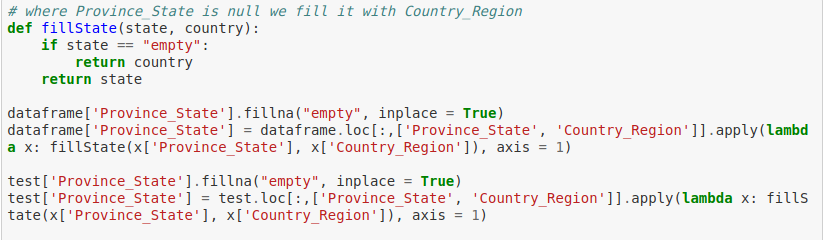
\includegraphics[scale=0.5]{pretprocesiranje1.png}
    \caption{Popunjavanje nedostajućih vrednosti}
    \label{fig:Pretprocesiranje1}
\end{figure}

Kada mreža koristi podatke koji su u velikom rasponu vrednosti, za velike ulaze može doći do velikog usporavanja učenja kao i konvergencije, stoga potrebno je skalirati date podatke. Postoje dva nacina za skaliranje vrednosti:

\begin{itemize}
    \item \textbf{Normalizacija}: Ponovno skaliranje vrednosti podataka tako da su svi u opsegu od 0 do 1.
    \item \textbf{Standardizacija}: Reskaliranje vrednosti podataka tako da je srednja vrednost 0 a standardna devijacija 1.
\end{itemize}

Za potrebe ovog projekta korisćena je normalizacija (Standardizaciju ima smisla koristiti kada bi imali Gausovu raspodelu). Normalizaciju datog skupa podataka vršimo pomoću biblioteke scikit-learn i objekta MinMaxScaler.\ref{fig:Pretprocesiranje2}

\begin{figure}[htp]
    \centering
    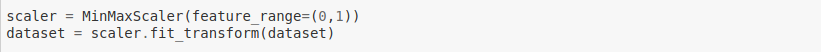
\includegraphics[scale=0.5]{pretprocesiranje2.png}
    \caption{Normalizacija podataka}
    \label{fig:Pretprocesiranje2}
\end{figure}



\subsection{Učenje modela nad trening podacima}
\subsection{Testiranje modela}


\section{Zaključak}
\label{sec:zakljucak}


\addcontentsline{toc}{section}{Literatura}
\appendix
\bibliography{seminarski.bib} 
\bibliographystyle{plain}

\appendix
\section{Dodatak}

\end{document}

